\chapter{Tính năng AI của hệ thống}
\textit{Chương này trình bày các tính năng AI cốt lõi của hệ thống, tập trung vào hai năng lực chính là đánh giá kỹ năng Speaking và đánh giá kỹ năng Writing. Đối với Speaking, nhóm đã hiện thực một nền tảng chuyên biệt mang tên \textbf{Lingriser} nhằm tổ chức lộ trình luyện nói, hội thoại với AI và phối hợp cùng giáo viên/mentor. Đối với Writing, hệ thống tập trung vào định hướng chấm điểm và phân tích bài viết để nâng cao hiệu quả học tập cho người dùng.}


\section{Tính năng AI cho Speaking -- Nền tảng Lingriser}

\textit{Lingriser là hệ thống luyện nói tiếng Anh tích hợp AI được xây dựng cho học sinh Việt Nam. Thay vì chỉ cung cấp một giao diện hội thoại đơn thuần, Lingriser đặt AI vào vai trò thực thể trung gian trong một chu trình học tập khép kín, kết nối giáo viên, học sinh, mentor và phụ huynh qua cùng một luồng dữ liệu có cấu trúc sư phạm.}

\subsection{Mục tiêu và kiến trúc tổng thể}

\subsubsection{Mục tiêu hệ thống}

Mục tiêu cốt lõi của mô-đun Speaking là xây dựng môi trường luyện nói có cấu trúc với ba đặc tính kỹ thuật chủ đạo:

\begin{enumerate}
    \item \textbf{Luyện tập có định hướng sư phạm:} AI không hoạt động độc lập mà nhận mục tiêu luyện nói (\textit{weekly focus}) từ giáo viên, sau đó nhúng mục tiêu đó vào system prompt để điều hướng nội dung hội thoại.
    \item \textbf{Vòng phản hồi khép kín:} Mỗi phiên nói tạo ra dữ liệu analytics (phiên âm, phát hiện khoảng ngừng, thời lượng phản hồi) được lưu vào cơ sở dữ liệu và kế thừa sang các bước học tiếp theo.
    \item \textbf{Tích hợp đa vai trò:} Dữ liệu AI sinh ra phục vụ đồng thời nhiều tác nhân -- học sinh luyện tập, giáo viên đặt mục tiêu, mentor đọc tóm tắt trước buổi gọi, phụ huynh theo dõi tiến độ.
\end{enumerate}

Mỗi khóa học được tổ chức thành \textbf{8 module hằng tuần}, mỗi module phân tầng hoạt động theo ngày:

\begin{table}[H]
\centering
\begin{tabular}{|l|l|p{7.5cm}|}
\hline
\textbf{Thời điểm} & \textbf{Hoạt động} & \textbf{Mô tả} \\ \hline
Thứ Hai & Học trực tiếp & Giáo viên giảng dạy và đặt \textit{weekly focus} -- mục tiêu luyện nói trọng tâm cho cả tuần \\ \hline
Thứ Ba -- Thứ Sáu & Luyện AI & Học sinh luyện nói với AI theo chủ đề và mục tiêu của giáo viên; hệ thống phiên âm, phản hồi và phát lại bằng giọng nói tổng hợp \\ \hline
Thứ Bảy -- Chủ Nhật & Gọi video & Buổi 1-on-1 với mentor bản ngữ qua Google Meet; mentor nhận \textit{mentor brief} tổng hợp từ kết quả luyện AI \\ \hline
\end{tabular}
\caption{Lịch trình hoạt động học tập hằng tuần trên Lingriser}
\end{table}

Nền tảng phục vụ năm vai trò người dùng với phạm vi truy cập riêng biệt:

\begin{table}[H]
\centering
\begin{tabular}{|l|p{9.5cm}|}
\hline
\textbf{Vai trò} & \textbf{Phạm vi chức năng} \\ \hline
\texttt{student} & Dashboard cá nhân, luyện nói với AI, đặt lịch video call, theo dõi tiến trình theo module \\ \hline
\texttt{teacher} & Dạy lớp thứ Hai, đặt \textit{weekly focus} để định hướng AI practice và mentor \\ \hline
\texttt{mentor} & Thực hiện buổi gọi video cuối tuần, xem \textit{mentor brief} tổng hợp từ kết quả luyện AI \\ \hline
\texttt{parent} & Theo dõi lịch học, mức độ tham gia luyện AI và chỉ báo tiến bộ hằng tuần của con \\ \hline
\texttt{admin} & Quản lý toàn bộ người dùng, khóa học, chương trình học và thống kê nền tảng \\ \hline
\end{tabular}
\caption{Các vai trò người dùng trên nền tảng Lingriser}
\end{table}

\subsection{Hiện thực các thành phần AI cốt lõi}

Mô-đun AI Practice được hiện thực trong \texttt{AIPracticeService} (NestJS), giao tiếp trực tiếp với OpenAI API qua SDK chính thức. Bốn endpoint tương ứng với bốn tác vụ AI độc lập:

\begin{table}[H]
\centering
\begin{tabular}{|l|l|p{6cm}|}
\hline
\textbf{Method} & \textbf{Endpoint} & \textbf{Chức năng} \\ \hline
POST & \texttt{/api/ai-practice/chat} & Hội thoại GPT-4o-mini (non-streaming) \\ \hline
POST & \texttt{/api/ai-practice/transcribe} & Phiên âm audio Whisper-1 (multipart) \\ \hline
POST & \texttt{/api/ai-practice/tts} & Chuyển văn bản thành giọng nói MP3 \\ \hline
POST & \texttt{/api/ai-practice/feedback} & Sinh phân tích buổi luyện từ transcript \\ \hline
\end{tabular}
\caption{Các API endpoint của mô-đun AI Practice}
\end{table}

\subsubsection{Hệ thống hội thoại và System Prompt Engineering}

Điểm kỹ thuật then chốt của mô-đun hội thoại là hàm \texttt{buildSystemPrompt()}, được gọi mỗi lần khởi tạo phiên luyện tập. Hàm này tổng hợp ngữ cảnh từ ba nguồn thành một system prompt duy nhất truyền vào GPT-4o-mini \cite{openai_gpt4o}:

\textbf{(1) Trình độ CEFR:} Mỗi level ánh xạ sang một bộ hướng dẫn ngôn ngữ cụ thể. Ví dụ, \texttt{beginner} → \textit{``Use simple vocabulary and short sentences. Avoid complex grammar.''}, còn \texttt{advanced} → \textit{``Use rich vocabulary, complex grammar, and natural expressions like a native speaker.''}. Tham số \texttt{temperature = 0.8} và \texttt{max\_tokens = 500} được cố định để đảm bảo phản hồi đa dạng nhưng có độ dài phù hợp.

\textbf{(2) Weekly Focus Goals:} Nếu mảng \texttt{speakingGoals[]} từ bảng \texttt{weekly\_focus} không rỗng, từng mục tiêu được nối thành khối \texttt{WEEKLY SPEAKING GOALS} trong system prompt, kèm hướng dẫn để AI dẫn dắt hội thoại về phía các mục tiêu đó. Đây là cơ chế kỹ thuật trực tiếp kết nối dữ liệu của giáo viên với hành vi của mô hình ngôn ngữ.

\textbf{(3) Quy tắc hội thoại nghiêm ngặt:} System prompt mã hóa bốn ràng buộc cứng: (a) bám sát chủ đề, tối đa một câu follow-up về chi tiết phụ rồi quay lại chủ đề chính; (b) không bình luận dài dòng, chỉ hỏi câu tiếp theo; (c) phản hồi tối đa 1--2 câu; (d) cuối mỗi lượt trả về 2--3 câu gợi ý định dạng JSON với key \texttt{suggestions}, kẹp giữa hai marker cố định \texttt{---SUGGESTIONS---} và \texttt{---END---}. Frontend parse khối này để hiển thị gợi ý tách biệt với nội dung hội thoại.

\subsubsection{Xử lý Speech-to-Text với Whisper}

Khi học sinh gửi audio, backend gọi Whisper-1 \cite{openai_whisper} với cấu hình:

\begin{itemize}
    \item \texttt{response\_format: 'verbose\_json'}: nhận timestamp cấp độ từng từ thay vì chỉ chuỗi văn bản.
    \item \texttt{timestamp\_granularities: ['word']}: kích hoạt trường \texttt{words[]} chứa \texttt{start} và \texttt{end} của từng từ, phục vụ cho các xử lý hạ nguồn như Pause Detection và tính \texttt{response\_duration}.
    \item Whisper được truyền vào một prompt hướng dẫn phiên âm nguyên văn, không tự động sửa lỗi phát âm, không bổ sung từ thiếu -- nhằm bảo toàn các lỗi thực tế của học sinh để phân tích.
\end{itemize}

Dữ liệu \texttt{words[]} từ Whisper là đầu vào duy nhất cho các thuật toán phân tích trong mục tiếp theo.

\subsubsection{Tổng hợp tiếng nói và vòng lặp nghe--nói}

Phản hồi văn bản từ GPT-4o-mini được chuyển thành giọng nói qua \texttt{gpt-4o-mini-tts} với giọng \texttt{alloy}, định dạng MP3. Backend trả buffer MP3 trực tiếp trong response body (\texttt{Content-Type: audio/mpeg}). Frontend nhận và phát âm thanh ngay lập tức, tạo vòng lặp nghe--nói liên tục mà không cần tải file xuống thiết bị. Chiến lược stream trực tiếp qua buffer này giúp giảm độ trễ cảm nhận (perceived latency) so với phương án lưu file tạm trên server.

\subsection{Thuật toán và xử lý dữ liệu đặc thù}

\subsubsection{Thuật toán Pause Detection}

Sau khi Whisper trả về danh sách \texttt{words[]} với timestamp từng từ, thuật toán Pause Detection được thực thi trong \texttt{generateFeedback()} để phát hiện khoảng ngừng trong phát biểu của học sinh.

Khoảng lặng $\text{gap}$ giữa hai từ liên tiếp $w_{i-1}$ và $w_i$ được xác định bởi:

$$\text{gap} = w_i.\text{start} - w_{i-1}.\text{end}$$

Thuật toán duyệt tuần tự qua \texttt{words[]} và áp dụng quy tắc:

\begin{enumerate}
    \item Nếu $\text{gap} > 0.5$ giây: tăng \texttt{pauseCount}, đánh dấu lượt đó vào \texttt{pauseTurns[]}, chèn marker \texttt{"uhmmm"} vào bản phiên âm để phản ánh khoảng ngừng thực tế.
    \item Kết quả được lưu vào cột \texttt{pause\_detection JSONB} của bảng \texttt{ai\_feedback}, gồm các trường: \texttt{has\_pause} (boolean), \texttt{pause\_count} (int), \texttt{pause\_turns[]} (mảng ID lượt có khoảng ngừng) và \texttt{summary} (mô tả bằng tiếng Việt).
\end{enumerate}

Ngưỡng $0.5$ giây được lựa chọn dựa trên đặc trưng ngôn ngữ học: khoảng lặng dưới ngưỡng này thường là ranh giới tự nhiên giữa các từ trong tiếng Anh liên tục, không phải dấu hiệu do dự.

\subsubsection{Phân tích Analytics: Response Duration và WPM}

Ngoài pause detection, hệ thống còn tính hai chỉ số bổ sung:

\textbf{Response Duration:} Thời gian phát biểu trung bình mỗi lượt, đo bằng cách lấy timestamp của từ cuối trừ timestamp của từ đầu:

$$\text{response\_duration} = w_{\text{last}}.\text{end} - w_0.\text{start}$$

\textbf{Ước lượng tốc độ nói (WPM):} Nếu không có dữ liệu timestamp (chế độ chat text thuần), hệ thống ước lượng thời lượng theo tốc độ phát biểu trung bình $2{,}2$ từ/giây. Toàn bộ analytics được gắn với bản ghi \texttt{learning\_history} tương ứng để phục vụ thống kê trên dashboard và \textit{mentor brief}.

\subsection{Thiết kế cơ sở dữ liệu và luồng dữ liệu}

\subsubsection{Data Modeling}

Lingriser sử dụng PostgreSQL (Neon Serverless) với schema quản lý hoàn toàn bằng file SQL thuần -- TypeORM được cấu hình \texttt{synchronize: false} để tránh auto-migration không kiểm soát.

\textbf{Pattern Single-table Base + Profile Extension} được áp dụng cho quản lý người dùng: bảng \texttt{users} lưu thông tin xác thực chung (\texttt{email}, \texttt{password\_hash}, \texttt{phone}, \texttt{role}, \texttt{is\_locked}); mỗi vai trò có bảng profile riêng quan hệ 1:1 qua khóa ngoại \texttt{user\_id ON DELETE CASCADE}. Bảng \texttt{students} mở rộng với \texttt{grade}, \texttt{cefr\_level} và \texttt{assigned\_inperson\_teacher\_id}; bảng \texttt{teachers} thêm \texttt{teacher\_type} (\texttt{in\_person} / \texttt{video\_call} / \texttt{both}), \texttt{bio} và \texttt{specialties}.

Quan hệ phụ huynh--học sinh không lưu bằng FK trực tiếp mà qua bảng trung gian \texttt{account\_links(student\_id, linked\_user\_id, link\_type)}, cho phép một phụ huynh theo dõi nhiều học sinh và một học sinh có nhiều phụ huynh; đồng thời tái sử dụng cho quan hệ giáo viên--học sinh với \texttt{link\_type = 'teacher'}.

\textbf{Lý do chọn JSONB cho dữ liệu AI:} Các trường phân tích như \texttt{pause\_detection} và nội dung module (\texttt{ai\_practice\_content}, \texttt{monday\_content}) được lưu dưới dạng JSONB. PostgreSQL JSONB hỗ trợ index GIN cho truy vấn nội bộ, đồng thời cho phép schema linh hoạt khi cấu trúc phản hồi AI thay đổi theo phiên bản mà không cần migration toàn bộ bảng.

Bảng \texttt{ai\_feedback} có quan hệ 1:1 với \texttt{learning\_history}, lưu bốn trường analytics: \texttt{speech\_to\_text} (bản phiên âm đầy đủ), \texttt{response\_duration} (giây trung bình mỗi lượt), \texttt{pause\_detection JSONB} (kết quả phát hiện khoảng ngừng) và \texttt{session\_length} (số lượt hội thoại).

Bảng \texttt{weekly\_focus} là cầu nối kỹ thuật giữa ba tầng học tập. Ràng buộc \texttt{UNIQUE(module\_id, teacher\_id)} đảm bảo mỗi giáo viên chỉ có một bản mục tiêu cho mỗi module, và \texttt{WeeklyFocusService.createOrUpdate()} tận dụng constraint này để upsert thay vì insert/update riêng. Trường \texttt{speaking\_goals TEXT[]} lưu danh sách mục tiêu dạng mảng native PostgreSQL, được TypeORM ánh xạ thành \texttt{string[]} và truyền thẳng vào \texttt{buildSystemPrompt()}.

Schema định nghĩa 15 index phủ các truy vấn thường xuyên nhất. Bảng \texttt{bookings} có ba index riêng trên \texttt{student\_id}, \texttt{booking\_date} và \texttt{status}; bảng \texttt{learning\_history} có index trên \texttt{student\_id} và \texttt{activity\_type} để phục vụ truy vấn thống kê tuần mà không cần full table scan.

\subsubsection{Pipeline dữ liệu: WeeklyFocus $\rightarrow$ AI Practice $\rightarrow$ Mentor Brief}

Đây là luồng dữ liệu kỹ thuật trung tâm của Lingriser, kết nối ba tầng hoạt động thành một chu trình có trạng thái. Toàn bộ pipeline không có bước thủ công nào giữa các tầng -- dữ liệu từ giáo viên tự động xuất hiện trong AI practice, và kết quả AI practice tự động tổng hợp thành mentor brief, nhờ các foreign key và truy vấn có cấu trúc trên cùng một PostgreSQL database.

\begin{enumerate}
    \item \textbf{Giáo viên thiết lập mục tiêu:} Giao diện quản lý gửi payload chứa định danh module, giáo viên, chủ đề và danh sách mục tiêu luyện nói. Backend thực hiện \textit{upsert} dựa trên ràng buộc \texttt{UNIQUE(module\_id, teacher\_id)}, lưu mảng \texttt{speaking\_goals TEXT[]} vào bảng \texttt{weekly\_focus}.

    \item \textbf{Tích hợp mục tiêu vào phiên AI:} Khi học sinh khởi tạo phiên luyện, client truyền danh sách mục tiêu trong payload. \texttt{AIPracticeService} gọi \texttt{buildSystemPrompt()}, nhúng mảng mục tiêu vào khối \texttt{WEEKLY SPEAKING GOALS} của system prompt. Mô hình ngôn ngữ sử dụng khối này như tập luật ràng buộc để điều hướng nội dung hội thoại.

    \item \textbf{Xử lý và lưu kết quả luyện tập:} Kết thúc phiên, hệ thống tạo bản ghi \texttt{learning\_history} với \texttt{activity\_type = 'ai\_practice'}. Luồng phân tích xử lý transcript để trích xuất pause detection và response duration, lưu vào \texttt{ai\_feedback} liên kết qua foreign key.

    \item \textbf{Tổng hợp Mentor Brief:} API tóm tắt thực thi các truy vấn song song: (a) truy xuất mục tiêu tuần từ \texttt{weekly\_focus}; (b) aggregation trên \texttt{learning\_history} xác định tần suất luyện tập; (c) JOIN để lấy dữ liệu đánh giá của phiên gần nhất. Kết quả đóng gói thành một response duy nhất để mentor đọc trước buổi video call.
\end{enumerate}

\subsection{Các mô-đun tích hợp hỗ trợ}

\subsubsection{Booking System -- Quản lý vòng đời buổi học}

Bảng \texttt{bookings} quản lý buổi video call qua hai enum độc lập tạo thành một State Machine:

\begin{itemize}
    \item \textbf{booking status} (\texttt{confirmed → completed / cancelled / no\_show}): theo dõi kết quả cuối cùng của buổi học.
    \item \textbf{meeting status} (\texttt{pending → in\_progress → ended}): theo dõi trạng thái thời gian thực trong buổi học.
\end{itemize}

Hai enum độc lập cho phép hệ thống phân biệt rõ giữa kết quả hành chính (booking có hoàn thành không) và trạng thái vận hành (buổi học đang ở giai đoạn nào). Khi buổi học bắt đầu, backend tạo link Google Meet tự động và lưu \texttt{meeting\_link} cùng \texttt{google\_event\_id} vào bảng. OAuth tokens của giáo viên lưu riêng trong \texttt{teacher\_google\_tokens} với cơ chế refresh tự động. Mentor có thể nhận \textit{mentor brief} trước buổi gọi dựa trên module học, mục tiêu tuần và lịch sử luyện tập gần nhất của học sinh.

\subsubsection{Parental Monitoring -- Truy vấn thống kê theo thời gian thực}

Phụ huynh là vai trò đặc biệt: không tham gia học tập nhưng được cấp quyền đọc toàn bộ dữ liệu của con qua một lớp truy cập riêng. Quan hệ phụ huynh--học sinh được quản lý qua bảng trung gian \texttt{account\_links}. Toàn bộ phương thức trong \texttt{ParentsService} đều xác minh quyền sở hữu trước khi trả dữ liệu: kiểm tra \texttt{children.some(c => c.id === studentId)}; nếu không khớp, ném \texttt{NotFoundException} tại service layer trước khi xuống database.

Thống kê AI practice theo tuần được tính bằng truy vấn aggregation trên PostgreSQL:
\begin{itemize}
    \item \texttt{DATE\_TRUNC('week', start\_time)} để nhóm theo tuần.
    \item \texttt{COUNT(*)} đếm số buổi; \texttt{EXTRACT(EPOCH FROM (end\_time - start\_time)) / 60} tính tổng phút.
    \item Backend thực hiện bước \textbf{fill missing weeks}: duyệt 8 tuần gần nhất, điền \texttt{sessions = 0} và \texttt{minutes = 0} cho các tuần không có dữ liệu, tạo mảng đủ 8 phần tử sẵn sàng render trực tiếp thành biểu đồ cột (Recharts).
\end{itemize}

Module hiện tại của học sinh được tính động tại mỗi request qua \texttt{computeCurrentModuleNumber()}, so sánh ngày hiện tại với \texttt{week\_start\_date}/\texttt{week\_end\_date} của từng module -- không lưu cứng trong database để tránh cần scheduled job cập nhật.

Ngoài dữ liệu số, học sinh có thể upload video tự quay trước (\texttt{video\_type = 'before'}) và sau (\texttt{video\_type = 'after'}) khóa học, lưu trên AWS S3 với tiền tố \texttt{lingriser/student-videos/}. Phụ huynh xem cả hai video qua endpoint \texttt{/progress-videos}, tạo bằng chứng hữu hình về sự tiến bộ trong 8 tuần học.

\subsection{Kết luận mô-đun Speaking}

Lingriser thể hiện một hướng triển khai AI cho Speaking vượt ra ngoài chatbot hội thoại đơn thuần.
Để làm rõ phạm vi kỹ thuật, có thể mô tả hệ thống qua góc nhìn đầu vào -- đầu ra như sau.

\textbf{Đầu vào} của mô-đun gồm ba nguồn độc lập được tổng hợp tại thời điểm khởi tạo phiên luyện:

\begin{enumerate}
    \item \textit{Trình độ CEFR} của học sinh, xác định ngưỡng từ vựng và cấu trúc ngữ pháp mà AI sử dụng trong hội thoại.
    \item \textit{Weekly focus goals} do giáo viên đặt từ buổi học trực tiếp đầu tuần, được nhúng trực tiếp vào system prompt để định hướng nội dung hội thoại.
    \item \textit{Audio đầu vào} của học sinh tại mỗi lượt nói, được gửi lên backend dưới dạng multipart để xử lý phiên âm.
\end{enumerate}

\textbf{Đầu ra} của hệ thống phân tầng theo đối tượng thụ hưởng:

\begin{itemize}
    \item \textbf{Với học sinh:} Phản hồi hội thoại dạng văn bản và âm thanh tổng hợp (MP3) trả về ngay trong phiên, cùng các gợi ý câu định dạng JSON hiển thị song song giao diện.
    \item \textbf{Với hệ thống lưu trữ:} Mỗi phiên tạo ra bản ghi \texttt{ai\_feedback} gồm bản phiên âm đầy đủ (\texttt{speech\_to\_text}), chỉ số thời lượng phản hồi trung bình (\texttt{response\_duration}), kết quả phát hiện khoảng ngừng (\texttt{pause\_detection JSONB}) và tổng số lượt hội thoại (\texttt{session\_length}).
    \item \textbf{Với các tác nhân khác trong hệ sinh thái:} Mentor nhận \textit{mentor brief} tổng hợp tự động từ dữ liệu trên trước buổi video call; phụ huynh theo dõi biểu đồ tần suất luyện tập theo tuần và chỉ báo tiến bộ trên dashboard riêng.
\end{itemize}

Giá trị kỹ thuật của hệ thống nằm ở ba điểm:

\begin{enumerate}
    \item System Prompt Engineering cho phép nhúng ngữ cảnh sư phạm vào hành vi của LLM.
    \item Whisper với timestamp cấp từ tạo nền tảng cho các thuật toán phân tích ngôn ngữ hạ nguồn.
    \item Pipeline dữ liệu có cấu trúc biến mỗi phiên luyện tập thành đầu vào có ích cho các tác nhân khác trong hệ sinh thái.
\end{enumerate}

Từ góc độ kiến trúc, đây là minh chứng cụ thể cho khả năng tích hợp AI vào sản phẩm giáo dục
theo hướng vừa khả thi về kỹ thuật, vừa có giá trị sư phạm thực tiễn.

\section{Mô-đun chấm điểm và phản hồi IELTS Writing tự động}

Bên cạnh khả năng xử lý hội thoại thời gian thực của mô-đun Speaking, hệ thống được tích hợp thêm thành phần AI chuyên biệt cho tác vụ Writing. Khác với Speaking vốn trọng tâm là xử lý tín hiệu âm thanh, mô-đun Writing tập trung vào phân tích ngữ nghĩa, đánh giá chất lượng văn bản học thuật và sinh phản hồi định hướng cải thiện (formative feedback). Trong phạm vi đồ án, nhóm đã thực hiện tinh chỉnh (fine-tuning) mô hình ngôn ngữ lớn \textbf{Phi-3-mini-4k-instruct}, triển khai dưới dạng dịch vụ độc lập thông qua hạ tầng điện toán đám mây để cung cấp khả năng chấm điểm chính xác và tối ưu về mặt chi phí vận hành.

\subsection{Mục tiêu và bài toán xây dựng mô hình}
Mục tiêu cốt lõi của mô-đun là mô phỏng quy trình đánh giá bài viết của giám khảo chuyên môn, cung cấp một hệ thống phản hồi hai lớp:
\begin{itemize}
    \item \textbf{Đánh giá định lượng:} Dự đoán chính xác điểm tổng (\textit{Overall Band Score}) và điểm 4 tiêu chí thành phần (\textit{Task Achievement, Coherence \& Cohesion, Lexical Resource, Grammatical Range \& Accuracy}) theo thang điểm 9 truyền thống của IELTS.
    \item \textbf{Đánh giá định tính:} Sinh nhận xét chi tiết, chỉ rõ các điểm lỗi và gợi ý cách diễn đạt nâng cao, giúp người học tự điều chỉnh bài viết.
\end{itemize}

Về mặt kỹ thuật, đây là bài toán \textit{Instruction Tuning} đa nhiệm. Mô hình phải tiếp nhận đồng thời đề bài và bài làm, sau đó suy luận để đưa ra kết quả có cấu trúc (Structured Output). Nhóm lựa chọn \textbf{Phi-3-mini} (3.8B tham số) \cite{phi3_microsoft} làm mô hình nền do sự cân bằng tối ưu giữa kích thước và năng lực suy luận ngôn ngữ, đặc biệt là khả năng tương thích cao với kỹ thuật lượng tử hóa \textit{4-bit} giúp vận hành ổn định trên tài nguyên phần cứng hạn chế.

\subsection{Cơ sở lý thuyết}

\subsubsection{Mô hình ngôn ngữ lớn và dòng mô hình Phi-3}
Mô hình ngôn ngữ lớn (Large Language Models - LLMs) là các hệ thống học sâu dựa trên kiến trúc Transformer, được huấn luyện trên tập dữ liệu văn bản khổng lồ để hiểu và sinh ngôn ngữ tự nhiên. 

Trong đồ án này, nhóm sử dụng \textbf{Phi-3-mini-4k-instruct}, một mô hình ngôn ngữ nhỏ (Small Language Model - SLM) được phát triển bởi Microsoft. Phi-3-mini có các đặc điểm nổi bật phù hợp với bài toán thực tế của hệ thống:
\begin{itemize}
    \item \textbf{Kích thước tối ưu:} Với khoảng 3,8 tỷ tham số, mô hình đủ nhỏ để triển khai trên các tài nguyên phần cứng hạn chế (như GPU Tesla T4 hoặc CPU thông thường) nhưng vẫn duy trì năng lực suy luận tương đương các mô hình lớn hơn nhiều lần.
    \item \textbf{Dữ liệu huấn luyện tập trung:} Phi-3 được huấn luyện dựa trên tập dữ liệu tập trung vào tư duy logic và các văn bản giáo dục chất lượng cao, giúp nó có khả năng nắm bắt tốt các cấu trúc ngữ pháp và yêu cầu học thuật khắt khe của bài thi IELTS.
    \item \textbf{Ngữ cảnh hỗ trợ:} Phiên bản 4k hỗ trợ độ dài ngữ cảnh lên tới 4096 tokens, đáp ứng tốt yêu cầu xử lý đồng thời đề bài, chỉ dẫn chấm điểm và bài viết dài của thí sinh.
\end{itemize}

\subsubsection{Kỹ thuật tinh chỉnh tham số hiệu quả (PEFT) và QLoRA}
Việc huấn luyện lại toàn bộ hàng tỷ tham số của một mô hình ngôn ngữ (Full Fine-tuning) đòi hỏi tài nguyên tính toán cực lớn và dễ gây ra hiện tượng quên kiến thức cũ. Do đó, nhóm áp dụng kỹ thuật \textbf{PEFT (Parameter-Efficient Fine-Tuning)}, cụ thể là phương pháp \textbf{QLoRA}.

\begin{enumerate}
    \item \textbf{LoRA (Low-Rank Adaptation):} Thay vì cập nhật toàn bộ ma trận trọng số gốc, LoRA đóng băng mô hình nền và chỉ huấn luyện các cặp ma trận thứ hạng thấp (low-rank matrices) được thêm vào các lớp Transformer. Điều này làm giảm số lượng tham số cần cập nhật xuống mức tối thiểu (dưới 2\%) mà vẫn đạt hiệu quả tương đương \cite{lora_hu}.
    \item \textbf{Quantization (Lượng tử hóa 4-bit):} QLoRA đưa các trọng số của mô hình từ định dạng 16-bit xuống còn 4-bit (NormalFloat4). Kỹ thuật này giúp giảm đáng kể mức tiêu thụ VRAM, cho phép thực hiện tinh chỉnh mô hình trên các GPU phổ thông như Tesla T4 \cite{qlora}.
    \item \textbf{Tối ưu hóa với Unsloth:} Nhóm sử dụng thư viện Unsloth để thực thi thuật toán. Đây là framework giúp tăng tốc độ huấn luyện gấp 2 lần và tối ưu hóa việc quản lý bộ nhớ, giúp quá trình hội tụ của mô hình diễn ra nhanh chóng và ổn định hơn.
\end{enumerate}

\subsubsection{Lượng tử hóa mô hình và định dạng GGUF}
Sau khi huấn luyện, mô hình cần được tối ưu hóa để phục vụ giai đoạn triển khai (inference). Định dạng \textbf{GGUF (GPT-Generated Unified Format)} được nhóm lựa chọn nhờ các ưu điểm:
\begin{itemize}
    \item \textbf{Tính linh hoạt cao:} GGUF cho phép mô hình chạy mượt mà trên cả CPU và GPU. Cơ chế \textit{GPU Offloading} cho phép tận dụng tối đa sức mạnh phần cứng có sẵn để tăng tốc độ nhả chữ (tokens per second).
    \item \textbf{Nén dung lượng hiệu quả:} Thông qua phương pháp lượng tử hóa Q4\_K\_M, mô hình được nén xuống còn khoảng 2,32 GB. Điều này không chỉ tiết kiệm không gian lưu trữ mà còn giảm thiểu thời gian chờ khi hệ thống khởi động máy chủ (Cold-start).
\end{itemize}

\subsubsection{Kiến trúc hướng sự kiện và Hàng đợi thông điệp (Message Queue)}
Do đặc thù các tác vụ AI thường tốn nhiều thời gian xử lý (từ 30 giây đến vài phút), việc sử dụng kiến trúc đồng bộ truyền thống sẽ gây treo hệ thống. Nhóm đã áp dụng kiến trúc \textbf{hướng sự kiện (Event-driven)}:

\begin{itemize}
    \item \textbf{RabbitMQ:} Đóng vai trò là hàng đợi (Queue) điều phối thông điệp. Khi người dùng nộp bài, yêu cầu được đóng gói và gửi vào hàng đợi thay vì bắt trình duyệt phải giữ kết nối mở lâu.
    \item \textbf{Xử lý bất đồng bộ (Asynchronous):} Worker AI sẽ chủ động lấy yêu cầu từ hàng đợi để xử lý khi có tài nguyên rảnh. Cách tiếp cận này giúp hệ thống có khả năng mở rộng tốt (Scalability) và chịu tải cao khi có nhiều người dùng cùng lúc.
    \item \textbf{Tính bền vững (Resilience):} Hàng đợi cho phép hệ thống tự động thử lại (Retry) nếu gặp lỗi kết nối tạm thời tới AI Endpoint, đảm bảo bài viết của người dùng luôn được chấm điểm thành công.
\end{itemize}

\subsection{Xây dựng và tiền xử lý dữ liệu huấn luyện}

\subsubsection{Nguồn dữ liệu và Pipeline chuẩn hóa}
Dữ liệu huấn luyện được tổng hợp từ bốn nguồn uy tín nhằm đảm bảo độ bao phủ về cả Task 1 (biểu đồ) và Task 2 (nghị luận):
\begin{itemize}
    \item \textbf{Kaggle IELTS Dataset:} Cung cấp cấu trúc bài viết và điểm số ổn định.
    \item \textbf{Hugging Face (chillies/IELTS-writing-task-2-evaluation):} Nguồn dữ liệu quý giá kết hợp bài viết thực của thí sinh, điểm từ chuyên gia và phản hồi chi tiết được hỗ trợ sinh bởi Gemini Pro.
    \item \textbf{IELTS Mentor \& IELTS Blog:} Bổ sung các mẫu bài làm ở đa dạng các dải điểm (\textit{band scores}) và chủ đề thực tế.
\end{itemize}

Dữ liệu thô sau khi thu thập (9872 bản ghi) được đưa qua quy trình làm sạch nghiêm ngặt. Nhóm thực hiện lọc bỏ các mẫu thiếu điểm thành phần hoặc có phần phản hồi quá ngắn (dưới 50 ký tự), thu được tập dữ liệu tinh lọc gồm \textbf{7614} mẫu.

\subsubsection{Đặc trưng dữ liệu và Chat Template}
Để mô hình hóa tác vụ chấm điểm dưới dạng một cuộc hội thoại, dữ liệu được cấu trúc hóa theo định dạng message:
\begin{itemize}
    \item \textbf{System Prompt:} Định nghĩa vai trò ``IELTS Academic Writing Tutor'', cung cấp các chỉ dẫn về tiêu chí chấm điểm (\textit{Band Descriptors}).
    \item \textbf{User Prompt:} Gồm phân loại Task, nội dung đề bài và bài viết của người học.
    \item \textbf{Assistant Response:} Kết quả kỳ vọng gồm bảng điểm định dạng Markdown và phần nhận xét chi tiết.
\end{itemize}

Toàn bộ tập dữ liệu sau khi định dạng có độ dài trung bình khoảng \textbf{1028 tokens}, hoàn toàn nằm trong ngưỡng ngữ cảnh (\textit{Context Window}) 4096 tokens của Phi-3, đảm bảo không xảy ra hiện tượng mất mát thông tin trong quá trình huấn luyện.

\begin{figure}[H]
    \centering
    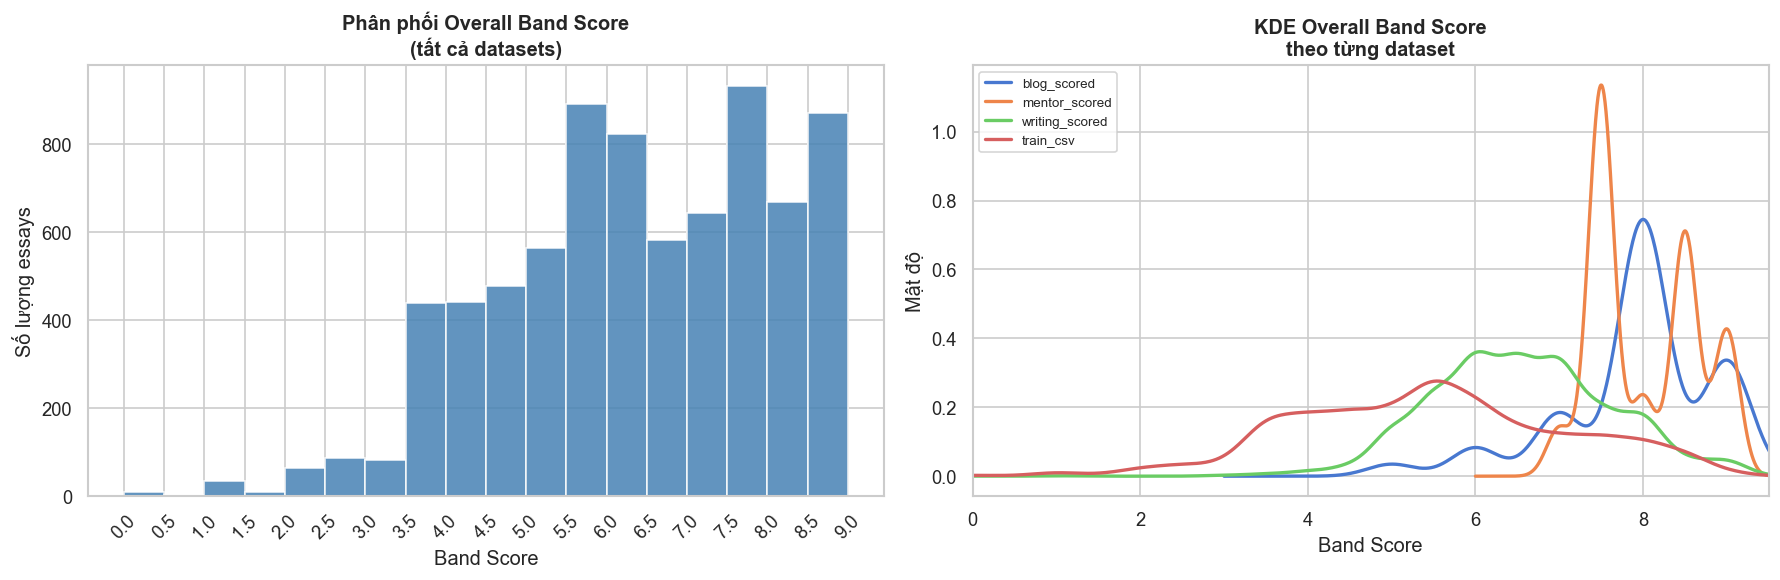
\includegraphics[width=0.82\linewidth]{graphics/writing/phan_phoi_data_set}
    \caption{Phân phối Overall Band Score}
\end{figure}

\begin{figure}[H]
    \centering
    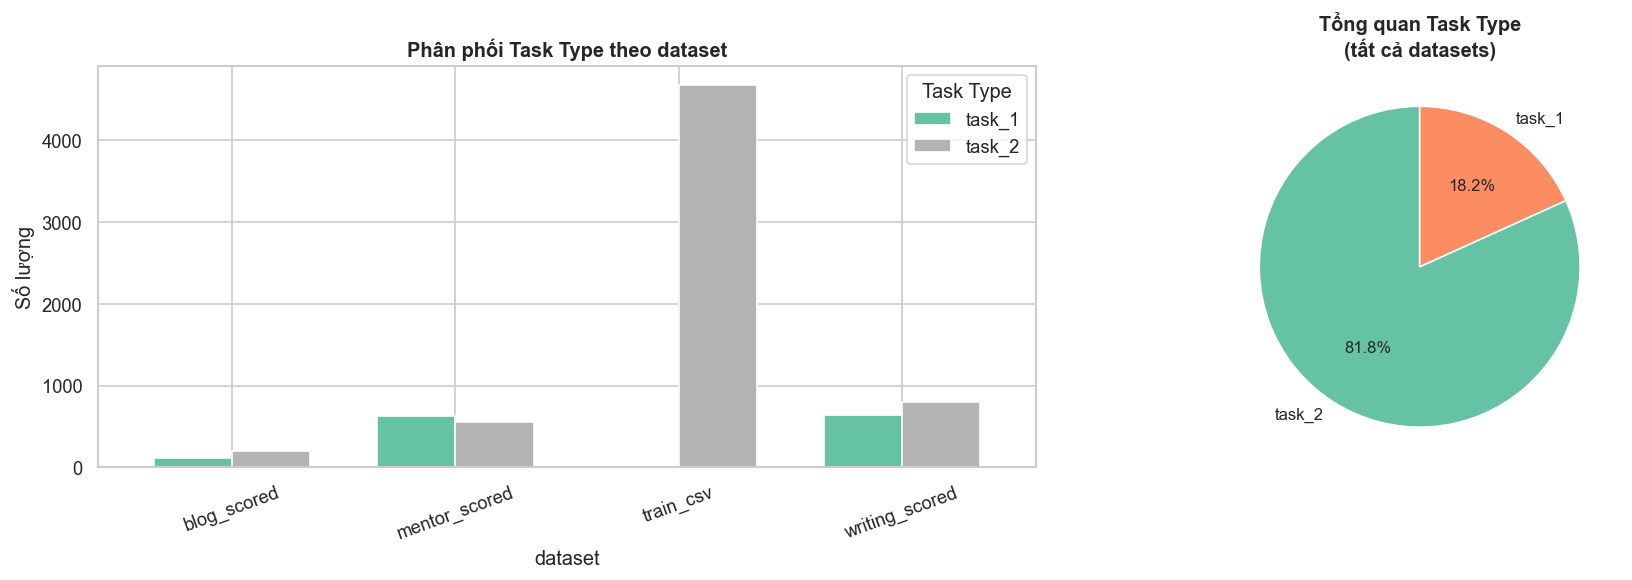
\includegraphics[width=0.82\linewidth]{graphics/writing/phan_phoi_task_type}
    \caption{Phân phối Task Type (Task 1 vs Task 2)}
\end{figure}

\subsection{Chiến lược huấn luyện và Tối ưu hóa}
Nhóm áp dụng kỹ thuật \textbf{QLoRA} \cite{qlora} kết hợp với thư viện \textbf{Unsloth} nhằm tối ưu hóa tốc độ huấn luyện và giảm thiểu tiêu thụ VRAM trên GPU Tesla T4 của Kaggle.

\begin{table}[H]
\centering
\caption{Cấu hình siêu tham số huấn luyện (Hyperparameters)}
\begin{tabular}{|l|l||l|l|}
\hline
\textbf{Tham số} & \textbf{Giá trị} & \textbf{Tham số} & \textbf{Giá trị} \\ \hline
Base Model & Phi-3-mini-4bit & Optimizer & AdamW 8-bit \\ \hline
LoRA Rank (r) & 16 & Learning Rate & 2e-4 \\ \hline
LoRA Alpha & 16 & LR Scheduler & Cosine \\ \hline
Batch Size hiệu dụng & 8 & Num Epochs & 3 \\ \hline
\end{tabular}
\end{table}

Việc chỉ cập nhật \textbf{1.47\%} tham số (khoảng 29.9M tham số LoRA adapters) cho phép mô hình học được đặc trưng của bài thi IELTS mà không làm mất đi tri thức tổng quát đã có. Quá trình huấn luyện kéo dài khoảng 7 giờ, đạt mức \textit{Final Train Loss} là \textbf{0.8757}, cho thấy sự hội tụ tốt của mô hình trên tập dữ liệu chuyên biệt.

\subsection{Kiến trúc triển khai và Quy trình suy luận}

\subsubsection{Hạ tầng Hugging Face Inference Endpoints}
Sau khi huấn luyện, mô hình được chuyển đổi sang định dạng \textbf{GGUF} nhằm giảm dung lượng tệp tin xuống còn khoảng \textbf{2.32 GB}, cho phép triển khai linh hoạt trên cả CPU và GPU. Nhóm lựa chọn giải pháp \textbf{Hugging Face Inference Endpoints} kết hợp với chiến lược \textbf{Scale-to-Zero}. Cấu hình này cho phép máy chủ tự động ngủ đông sau một thời gian không có lưu lượng truy cập, giúp tối ưu hóa chi phí vận hành cho đồ án thực tế.

\subsubsection{Cơ chế xử lý bất đồng bộ với RabbitMQ}
Do đặc thù các bài viết IELTS thường dài và việc suy luận mô hình ngôn ngữ lớn trên CPU có độ trễ nhất định (từ 1-2 phút), nhóm đã thiết kế một \textbf{Writing Service} đóng vai trò trung gian sử dụng kiến trúc hướng sự kiện (\textit{Event-driven}):
\begin{enumerate}
    \item \textbf{Tiếp nhận:} Backend chính nhận bài viết từ người dùng và đẩy thông điệp vào hàng đợi \textbf{RabbitMQ}.
    \item \textbf{Xử lý ngầm:} Worker AI lấy thông điệp từ hàng đợi, thực hiện tiền xử lý và gọi API tới Hugging Face Endpoint.
    \item \textbf{Phản hồi:} Kết quả sau khi AI chấm xong được gửi ngược lại qua hàng đợi kết quả để cập nhật vào cơ sở dữ liệu và thông báo cho người dùng.
\end{enumerate}
Kiến trúc này giúp tách rời (\textit{decoupling}) các thành phần hệ thống, đảm bảo Backend không bị treo trong quá trình chờ AI phản hồi và tăng khả năng chịu tải (\textit{scalability}) khi có nhiều người dùng đồng thời.

\subsection{Kết quả thực nghiệm và Đánh giá}
Để kiểm chứng hiệu quả của việc fine-tune, nhóm thực hiện đánh giá so sánh trực tiếp giữa mô hình \textbf{Phi-3 SFT} và mô hình thương mại \textbf{GPT-4o-mini} trên tập dữ liệu kiểm thử độc lập. Các chỉ số đo lường tập trung vào độ lệch band điểm thực tế.

\begin{table}[H]
\centering
\caption{So sánh hiệu năng giữa Phi-3 SFT và GPT-4o-mini}
\renewcommand{\arraystretch}{1.3}
\small
\begin{tabular}{|p{0.28\linewidth}|>{\centering\arraybackslash}p{0.20\linewidth}|>{\centering\arraybackslash}p{0.14\linewidth}|p{0.24\linewidth}|}
\hline
\textbf{Chỉ số (Metric)} & \textbf{Phi-3 SFT (Nhóm build)} & \textbf{GPT-4o-mini} & \textbf{Ý nghĩa} \\ \hline
MAE (Mean Absolute Error) & \textbf{0.976} & 1.205 & Sai số band điểm (càng thấp càng tốt) \\ \hline
RMSE & \textbf{1.332} & 1.487 & Phạt các sai số lớn (càng thấp càng tốt) \\ \hline
Pearson Correlation (r) & \textbf{0.638} & 0.566 & Độ tương quan xu hướng (càng cao càng tốt) \\ \hline
Within 0.5 Band (\%) & \textbf{51.0\%} & 35.8\% & Tỉ lệ chấm gần sát thực tế \\ \hline
Bias & \textbf{+0.049} & -0.684 & Xu hướng chấm khắt khe/nới lỏng \\ \hline
\end{tabular}
\end{table}

Kết quả cho thấy mô hình Phi-3 sau khi được huấn luyện chuyên biệt cho kết quả vượt trội hơn mô hình tổng quát GPT-4o-mini ở hầu hết các khía cạnh, đặc biệt là ở chỉ số \textbf{MAE} và \textbf{Within 0.5 Band}. Điều này minh chứng rằng việc fine-tune trên dữ liệu chuyên miền (\textit{domain-specific}) giúp AI hiểu sâu sắc các tiêu chí chấm điểm đặc thù của IELTS hơn các mô hình đa năng.

\subsection{Kết luận mô-đun}
Mô-đun Writing đã hiện thực hóa thành công quy trình từ thu thập dữ liệu, huấn luyện mô hình ngôn ngữ lớn đến triển khai hệ thống thực tế. Việc kết hợp công nghệ QLoRA và kiến trúc hàng đợi RabbitMQ không chỉ giải quyết bài toán chất lượng chấm điểm mà còn đảm bảo tính kinh tế và ổn định kỹ thuật cho hệ thống luyện thi tiếng Anh của nhóm.

\section{Kết luận chương}
Chương này cho thấy AI trong hệ thống không chỉ được dùng như một thành phần bổ sung, mà đóng vai trò trung tâm trong việc thiết kế trải nghiệm học tập. Với kỹ năng Speaking, Lingriser là minh họa rõ nét cho cách kết hợp hội thoại AI, phiên âm, tổng hợp tiếng nói, theo dõi tiến trình và điều phối sư phạm trong một nền tảng thống nhất. Với kỹ năng Writing, hệ thống định hướng khai thác AI để phân tích bài viết và chấm điểm theo tiêu chí band score.

Việc tách riêng hai hướng Speaking và Writing giúp làm rõ đặc thù dữ liệu, mục tiêu đánh giá và cách tích hợp AI cho từng kỹ năng. Đồng thời, chương này cũng tạo cơ sở để các phần sau có thể tiếp tục đánh giá sâu hơn về hiệu quả, khả năng mở rộng và giá trị thực tiễn của các mô-đun AI trong toàn bộ hệ thống.